% Politecnico di Milano (PoliMi) - School of Industrial and Information Engineering
%
% Copyright 2021 Politecnico di Milano, Italy. Inc. NC-BY

\documentclass[11pt,a4paper]{article} 

%------------------------------------------------------------------------------
%	REQUIRED PACKAGES AND  CONFIGURATIONS
%------------------------------------------------------------------------------
% PACKAGES FOR TITLES
\usepackage{titlesec}
\usepackage{color}

% PACKAGES FOR LANGUAGE AND FONT
\usepackage[utf8]{inputenc}
\usepackage[english]{babel}
\usepackage[T1]{fontenc} % Font encoding

% PACKAGES FOR IMAGES
\usepackage{graphicx}
\graphicspath{{Images/}}
\usepackage{eso-pic} % For the background picture on the title page
\usepackage{subfig} % Numbered and caption subfigures using \subfloat
\usepackage{caption} % Coloured captions
\usepackage{transparent}

% STANDARD MATH PACKAGES
\usepackage{amsmath}
\usepackage{amsthm}
\usepackage{bm}
\usepackage[overload]{empheq}  % For braced-style systems of equations

% PACKAGES FOR TABLES
\usepackage{tabularx}
\usepackage{longtable} % tables that can span several pages
\usepackage{colortbl}
\usepackage{array}
\usepackage{rotating}
\usepackage{afterpage}

% PACKAGES FOR ALGORITHMS (PSEUDO-CODE)
\usepackage{algorithm}
\usepackage{algorithmic}

% PACKAGES FOR REFERENCES & BIBLIOGRAPHY
\usepackage[colorlinks=true,linkcolor=black,anchorcolor=black,citecolor=black,filecolor=black,menucolor=black,runcolor=black,urlcolor=black]{hyperref} % Adds clickable links at references
\usepackage{cleveref}
\usepackage[sort&compress, square]{natbib} % Square brackets, citing references with numbers, citations sorted by appearance in the text and compressed
\bibliographystyle{unsrtnat} % You may use a different style adapted to your field DEFAULT: abbrvnat
%\setcitestyle{authoryear, square}
\setcitestyle{numbers, square}

% PACKAGES FOR THE APPENDIX
\usepackage{appendix}

% PACKAGES FOR ITEMIZE & ENUMERATES 
\usepackage{enumitem}

% OTHER PACKAGES
\usepackage{amsthm,thmtools,xcolor} % Coloured "Theorem"
\usepackage{comment} % Comment part of code
\usepackage{fancyhdr} % Fancy headers and footers
\usepackage{lipsum} % Insert dummy text
\usepackage{tcolorbox} % Create coloured boxes (e.g. the one for the key-words)

%-------------------------------------------------------------------------
%	NEW COMMANDS DEFINED
%-------------------------------------------------------------------------
% EXAMPLES OF NEW COMMANDS -> here you see how to define new commands
\newcommand{\bea}{\begin{eqnarray}} % Shortcut for equation arrays
\newcommand{\eea}{\end{eqnarray}}
\newcommand{\e}[1]{\times 10^{#1}}  % Powers of 10 notation
\newcommand{\mathbbm}[1]{\text{\usefont{U}{bbm}{m}{n}#1}} % From mathbbm.sty
\newcommand{\pdev}[2]{\frac{\partial#1}{\partial#2}}
% NB: you can also override some existing commands with the keyword \renewcommand

%----------------------------------------------------------------------------
%	ADD YOUR PACKAGES (be careful of package interaction)
%----------------------------------------------------------------------------
\usepackage{listings}

\colorlet{mygray}{black!30}
\colorlet{mygreen}{green!60!blue}
\colorlet{mymauve}{red!60!blue}

\lstset{
  backgroundcolor=\color{gray!10},  
  basicstyle=\ttfamily,
  columns=fullflexible,
  breakatwhitespace=false,      
  breaklines=true,                
  captionpos=b,                    
  commentstyle=\color{mygreen}, 
  extendedchars=true,              
  frame=single,                   
  keepspaces=true,             
  keywordstyle=\color{blue},      
  language=c++,                 
  numbers=none,                
  numbersep=5pt,                   
  numberstyle=\tiny\color{blue}, 
  rulecolor=\color{mygray},        
  showspaces=false,               
  showtabs=false,                 
  stepnumber=5,                  
  stringstyle=\color{mymauve},    
  tabsize=3,                      
  title=\lstname                
}%----------------------------------------------------------------------------
%	ADD YOUR DEFINITIONS AND COMMANDS (be careful of existing commands)
%----------------------------------------------------------------------------


% Do not change Configuration_files/config.tex file unless you really know what you are doing. 
% This file ends the configuration procedures (e.g. customizing commands, definition of new commands)
% Configuration package
\usepackage[bottom=2.0cm,top=2.0cm,left=2.0cm,right=2.0cm]{geometry}
\raggedbottom 

% Create color bluePoli (-> manuale grafica coordinata:  https://www.polimi.it/fileadmin/user_upload/il_Politecnico/grafica-coordinata/2015_05_11_46xy_manuale_grafica_coordinata.pdf)
\definecolor{bluePoli}{cmyk}{0.4,0.1,0,0.4}

% Custom theorem environments
\declaretheoremstyle[
  headfont=\color{bluePoli}\normalfont\bfseries,
  bodyfont=\color{black}\normalfont\itshape,
]{colored}

\captionsetup[figure]{labelfont={color=bluePoli}} % Set colour of the captions
\captionsetup[table]{labelfont={color=bluePoli}} % Set colour of the captions
\captionsetup[algorithm]{labelfont={color=bluePoli}} % Set colour of the captions

\theoremstyle{colored}
\newtheorem{theorem}{Theorem}[section]
\newtheorem{proposition}{Proposition}[section]

% Enhances the features of the standard "table" and "tabular" environments.
\newcommand\T{\rule{0pt}{2.6ex}}
\newcommand\B{\rule[-1.2ex]{0pt}{0pt}}

% Algorithm description
\newcounter{algsubstate}
\renewcommand{\thealgsubstate}{\alph{algsubstate}}
\newenvironment{algsubstates}{
    \setcounter{algsubstate}{0}%
    \renewcommand{\STATE}{%
    \stepcounter{algsubstate}%
    \Statex {\small\thealgsubstate:}\space}
    }{}
    
% Custom theorem environment
\newcolumntype{L}[1]{>{\raggedright\let\newline\\\arraybackslash\hspace{0pt}}m{#1}}
\newcolumntype{C}[1]{>{\centering\let\newline\\\arraybackslash\hspace{0pt}}m{#1}}
\newcolumntype{R}[1]{>{\raggedleft\let\newline\\\arraybackslash\hspace{0pt}}m{#1}}

% Custom itemize environment
\setlist[itemize,1]{label=$\bullet$}
\setlist[itemize,2]{label=$\circ$}
\setlist[itemize,3]{label=$-$}
\setlist{nosep}

% Create command for background pic
\newcommand\BackgroundPic{% Adding background picture
	\put(237,365){
	    \parbox[b][\paperheight]{\paperwidth}{%
	    \vfill
		\centering
		\transparent{0.4}
		
\includegraphics[width=0.44\paperwidth]{raggiera_polimi.eps}%
		\vfill}
		}
}

% Set indentation
\setlength\parindent{0pt}

% Custom title commands
\titleformat{\section}
{\color{bluePoli}\normalfont\Large\bfseries}
{\color{bluePoli}\thesection.}{1em}{}
\titlespacing*{\section}
{0pt}{3.3ex}{3.3ex}

\titleformat{\subsection}
{\color{bluePoli}\normalfont\large\bfseries}
{\color{bluePoli}\thesubsection.}{1em}{}
\titlespacing*{\subsection}
{0pt}{3.3ex}{3.3ex}

% Custom headers and footers
\pagestyle{fancy}
\fancyhf{}
      
\fancyfoot{}
\fancyfoot[C]{\thepage} % page
\renewcommand{\headrulewidth}{0mm} % headrule width
\renewcommand{\footrulewidth}{0mm} % footrule width

\makeatletter
\patchcmd{\headrule}{\hrule}{\color{black}\hrule}{}{} % headrule
\patchcmd{\footrule}{\hrule}{\color{black}\hrule}{}{} % footrule
\makeatother


% Insert here the info that will be displayed into your Title page 
% -> title of your work
\renewcommand{\title}{BUMP - BUbble column Multiphase Project}
% -> author name and surname
\renewcommand{\author}{Stefano Passoni, Martina Di Gennaro, Riccardo Giordani}
% -> abstract (only in English)
\renewcommand{\abstract}{}

% -> key-words (only in English)
\newcommand{\keywords}{here, the keywords, of your thesis}

\newcommand{\thead}[2][.95in]{%
  \vbox{\hsize#1\baselineskip11pt\centering\vspace*{3pt}#2\par}}

%-------------------------------------------------------------------------
%	BEGIN OF YOUR DOCUMENT
%-------------------------------------------------------------------------
\begin{document}

%-----------------------------------------------------------------------------
% TITLE PAGE
%-----------------------------------------------------------------------------
% Do not change Configuration_files/TitlePage.tex (Modify it IF AND ONLY IF you need to add or delete the Co-advisors)
% This file creates the Title Page of the document
% DO NOT REMOVE SPACES BETWEEN LINES!

\AddToShipoutPicture*{\BackgroundPic}

\hspace{-0.6cm}
\includegraphics[width=0.6\textwidth]{logo_polimi_ing_indinf.eps}

\vspace{-1mm}
\Large{\textbf{\color{bluePoli}{\title}}}\\

\vspace{-0.2cm}
\large{\textbf{\author}}

\small \normalfont

\vspace{11pt}

\centerline{\rule{1.0\textwidth}{0.4pt}}

%\begin{center}
%\begin{minipage}{.90 \textwidth}
%\noindent \textbf{\color{bluePoli} Abstract:} {\abstract}
%\end{minipage}
%\end{center}
\tableofcontents
\vspace{11pt}
\centerline{\rule{1.0\textwidth}{0.4pt}}
\vspace{15pt}

%\begin{tcolorbox}[arc=0pt, boxrule=0pt, colback=bluePoli!60, width=\textwidth, colupper=white]
  %  \textbf{Key-words:} Bubble column, Homogeneous flow regime, Computational fluid dynamics, Validation,
%\end{tcolorbox}

\vspace{12pt}




\section{Introduction}
\label{sec:1}
Bubble columns are multiphase reactors where the dispersed phase (gas) is introduced into a stationary or flowing liquid (continuous phase) and provide a good experimental setup to study the turbulent phenomena in dense bubbly flows. The functioning is apparently simple, as the ascending gas-phase creates a buoyancy-driven flow inducing the recirculation of the liquid phase. The local and the global fluid dynamic properties are related to the prevailing flow regime which may be homogeneous (bubbly flow condition at low superficial gas velocity, tipically $U_G<$ 0.03 $m/s$) or heterogeneous (churn-turbulent flow condition, $U_G>$ 0.1 $m/s$, $\alpha_G \geq$ 0.3). The homogeneous flow regime can be classified into the \textit{mono-dispersed homogeneous} flow regime, characterized by a mono-dispersed bubble size distribution (BSD), and the \textit{pseudo-homogeneous} flow regime, characterized by a poly-dispersed BSD. The distinction between mono-dispersed and poly-dispersed BSDs is based upon the change in the sign of the lift force coefficient. \\
Numerous industrial designs have been based on empirical correlations, but such approaches remain somewhat limited when increasing the reactor performance is sought. To improve the description of the physical phenomenon occurring in bubble columns a promising numerical method is the Computational Fluid Dynamics (CFD). CFD helps to understand the complex two-phase fluid dynamics in the bubble column through details of mean flows (fields of three components of mean velocities and mean gas hold-up), interphase rates of mass, energy and momentum transfer and turbulence parameters (such as turbulent kinetic energy, energy dissipation rate, Reynolds stresses, etc.). \\
In the present work, bubble column is numerically simulated by using the open source CFD tool OpenFOAM \cite{OF}. More in detail, the objective of this work is the validation of the already existing \textit{multiphaseEulerFoam} solver working for the case of \textit{mono-dispersed homogeneous} bubble column. For the case study we have considered a multiphase mixture of air and water without taking into account the heat transfer phenomena. \\
The structure of the report is as follows. In Section 2, the experimental benchmark taken as reference is illustrated. In Section 3, all details related to the numerical setup are delineated. In Section 4, the results are discussed. Conclusions and further development are outlined in Section 5.



\section{Experimental Benchmark}
\label{sec:2}
The  experimental benchmark taken as reference for the validation comes from the literature, in particular from the study of Krepper et al. \cite{krepper}. The experimental setup consists of three rectangular channels 20cm$^2$ in cross-section (0.1 × 0.02 $m$) bolted together at the flanges resulting in a bubble column of 1-meter height (Figure \ref{fig:facility}). The test facility is initially filled with water up to a specified (..) height. In the bottom of the test section is present a rectangular porous stone adopted as gas sparger 0.02$m$ wide, 0.01$m$ depth and 0.01$m$ height.This sparger produced a \textit{mono-dispersed homogeneous} bubble size distribution with a bubble diameter of 3-5 $mm$. The superficial gas flow rate, $U_G$, is varied between three different value, 0.006 $m/s$, 0.008 $m/s$ and 0.010 $m/s$, in the \textit{mono-dispersed homogenous} flow regime. The superficial velocity is calculated from the measured volume flow rates using: 
\begin{equation}
    U_G=\frac{Q_G}{A_{CS}}
\end{equation}
where $Q_G$ is the measured volume flow rate of the gas and $A_{CS}$ is the cross-sectional area of the test section. The column operates in the dispersed bubble bubbly regime, characterized by the absence of bubble coalescence or breakup, for the superficial gas velocities adopted in this work. For each superficial gas velocity the volume average void fraction, $\alpha_V$, also known as \textit{gas holdup}, can be calculated using: 
\begin{equation}
    \alpha_V=\frac{h_{final}-h_{initial}}{h_{final}}
\end{equation}
where $h_{final}$ is the heigth of the liquid column after the column has been aerated and $h_{initial}$ is the stationary height of the liquid column before aeration. The experimental data consist of wire-mesh local void fraction measurements performed at two different axial heights y = 0.08 $m$ and y = 0.63 $m$ above the gas sparger). The wire mesh sensor is placed in the cross-section by bolting it to two flanged rectangular channels. The wire-mesh sensor data was recorded at a frequency of 2500 Hz for a time period of 60 s. 
\begin{figure*}[!ht]
\centering
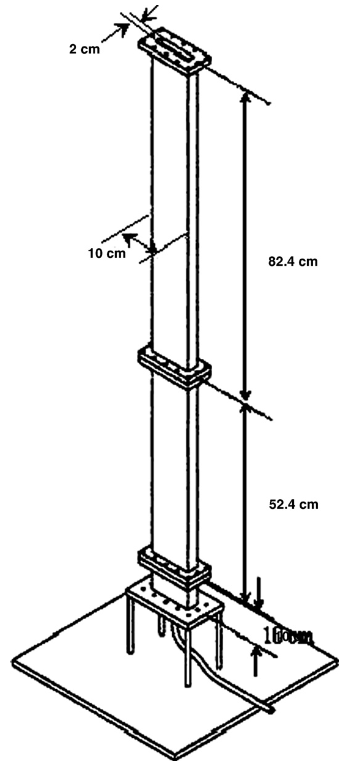
\includegraphics[width=4cm]{Report/Images/test facility.png}%
\caption{Dimensions and geometry of the experimental test facility.}
\label{fig:facility}
\end{figure*}

%-----------------------------------------------------------------------------
% NUMERICAL SETUP
%-----------------------------------------------------------------------------
\section{Numerical Setup}
\label{sec:numsetup}
In this section all the details related to the numerical setup will be presented and discussed.




\subsection{Domain and Mesh}
\label{sub:domain}
The numerical domain has been modeled and meshed with the utility \texttt{blockMesh} according to the size of the experimental facility reported in section \ref{sec:expbench}. The resulting mesh is structured and made of only regular hexahedral elements. Four different refinement levels were analyzed for the purpure of a grid sensitivity analysis. Figure \ref{fig:mesh} displays a section of the generated meshes and their details are instead summarized in table \ref{tab:meshes}. According to \cite{krepper}, the mesh size should be 1.5 times the size of the bubbles. Therefore, given the size distribution found in the experiments (see section \ref{sec:2}),  the coarsest mesh should be the most adequate since it has a cell size of 5mm in each direction. The grid refinement study has the purpose of verify if such a corse mesh has  negative influence on the fluid-dynamic phenomena inside the bubble column.

Speaking about the inlet section, the porous stone used as gas sparger in the experiments has been modeled as a zero-thickness surface having the size of the sparger itself, namely a 0.02x0.01 m\textsuperscript{2} cross-section.


\begin{figure}[H]
    \centering
    \subfloat[Mesh A]{
        \includegraphics[width=.25\textwidth, trim={250 0 250 0}, clip]{Images/mesh1.png}
    }
    \subfloat[Mesh B]{
        \includegraphics[width=.25\textwidth, trim={250 0 250 0}, clip]{Images/mesh2.png}
    }
    \subfloat[Mesh C]{
        \includegraphics[width=.25\textwidth, trim={250 0 250 0}, clip]{Images/mesh3.png}
    }
    \subfloat[Mesh D]{
        \includegraphics[width=.25\textwidth, trim={250 0 250 0}, clip]{Images/mesh4.png}
    }
    \caption[]{Different mesh densities considered in the analysis}
    \label{fig:mesh} 
\end{figure}

\begin{table}[H]
    \centering 
    \begin{tabular}{|p{5em} c c c c |}
    \hline
    \rowcolor{bluePoli!40}
    & \boldmath{$N_x$} & \boldmath{$N_y$} & \boldmath{$N_z$} & \textbf{Total no. of elements} \T\B \\
    \hline \hline
   \textbf{Mesh A} & 20 & 200 & 4 & 16000 \T\B \\
   \textbf{Mesh B} & 20 & 200 & 8 & 32000 \T\B \\
   \textbf{Mesh C} & 40 & 200 & 8 & 64000 \T\B \\
   \textbf{Mesh D} & 40 & 400 & 8 & 128000 \T\B \\
    \hline
    \end{tabular}
    \\[10pt]
    \caption{Mesh size details}
    \label{tab:meshes}
\end{table}



\subsection{Boundary Conditions}
\label{sub:bc}
The list of boundary conditions applied to the domain is summarized in table \ref{tab:bc}. At the inlet, three different gas superficial velocities were applied according to the three cases studied, respectively 6, 8 and 10 mm/s. These superficial velocities are an experimental input and were calculated as the volumetric flow rate of gas injected in the column divided by its volume. In OpenFOAM, a \texttt{flowRateInletVelocity} boundary condition was employed. This requires a mass flow rate input and a reference density in order to calculate the inlet velocity. The chosen density was 1.185 kg/m\textsuperscript{3} which corresponds to air density at ambient conditions of 25\textdegree C and 1 atm. \\


Moreover, a custom \texttt{fvModels} boundary condition was developed to implement a degassing boundary condition. The complete listing of the source code is provided in Appendix \ref{app:A}. Typically, a this type boundary condition is used to model a free surface through which dispersed gas bubbles are allowed to escape, but the continuous phase is not. A typical application is a bubble column in which the user want to reduce computational cost by not including the freeboard region in the simulation \cite{fluentuserguide}.  This boundary conditions offers also an improvement in terms of numerical stability since the water-air interface is not modeled. When the degassing boundary condition is specified for an outlet, the continuous liquid phase sees the boundary as a free-slip wall and does not leave the domain. The dispersed gas phase sees the boundary as an outlet. The code provided calculates an implicit mass source term to remove gas phase from the cells adjacent to the outlet boundary and also computes a degassing force to account for the effect of gas removal on the continuous phase.

% Table generated by Excel2LaTeX from sheet 'Foglio1'
\begin{table}[H]
  \centering
    \begin{tabular}{|p{5em} c c c|}
    \hline
    \rowcolor{bluePoli!40}
    \textbf{Variable} & \textbf{Inlet} & \textbf{Outlet} & \textbf{Walls} \T\B \\
     \hline \hline
    alpha.air & fixedValue & zeroGradient & zeroGradient \T\B \\
    alpha.water & fixedValue & zeroGradient & zeroGradient \T\B \\
    k.water & fixedValue & inletOutlet & kqRWallFunction \T\B \\
    epsilon.water & fixedValue & inletOutlet & epsilonWallFunction \T\B \\
    omega.water & fixedValue & inletOutlet & omegaWallFunction \T\B \\
    km    & fixedValue & inletOutlet & kqRWallFunction \T\B \\
    epsilonm & fixedValue & inletOutlet & epsilonWallFunction \T\B \\
    nut.water & calculated & calculated & nutkWallFunction \T\B \\
    p     & calculated & calculated & calculated \T\B \\
    U.air & flowRateInletVelocity & pressureInletOutletVelocity & fixedValue \T\B \\
    U.water & fixedValue & slip  & fixedValue \T\B \\
    \hline
    \end{tabular}%
  \caption{List of boundary conditions applied to the three different boundaries}
  \label{tab:bc}%
\end{table}%


\subsection{Working fluids and operating conditions}
\label{sub:fluids}
In order to model the bubble column, a two-phase mixture made of air and water was considered. As reported in section \ref{sec:2}, the experimental setup provided a monodispersed bubble size distribution with a mean equivalent diameter of 3mm. The dispersed phase is therefore modeled by using a single gas phase considering only small bubbles. Despite the air phase having a slightly varying density from the bottom to the top of the column, both fluids are considered incompressible. Table \ref{tab:materials} summarizes material properties of both phases. The column was simulated at ambient pressure of $10^5$ Pa with gravitational acceleration acting along Z coordinate. The system was considered isothermal and no thermophysical property was dependent on temperature. No heat nor mass transfer was considered between phases.

% Table generated by Excel2LaTeX from sheet 'Foglio1'
\begin{table}[H]
  \centering
    \begin{tabular}{|p{7em} c c c|}
    \hline
    \rowcolor{bluePoli!40}
    \textbf{Phase} & \textbf{Property} & \textbf{Type} & \textbf{Value} \T\B \\
     \hline \hline
    Air & Density & Constant & 1.185 [kg/m\textsuperscript{3}] \T\B \\
    Water & Density & Constant & 998.0 [kg/m\textsuperscript{3}] \T\B \\
    Air & Bubble diameter & Constant & 3 [mm] \T\B \\  
    Air and water & Surface Tension & Constant & 0.072 [N/m] \T\B \\   
    Air & E{ö}tv{ö}s number & Constant & 1    \T\B \\ 
    Air & Dynamic viscosity & Constant & 1.84e-05 [Pa/s]    \T\B \\ 
    Water & Dynamic viscosity & Constant & 3.65e-04 [Pa/s]    \T\B \\ 
    \hline
    \end{tabular}%
  \caption{List of boundary conditions applied to the three different boundaries}
  \label{tab:materials}%
\end{table}%



\subsection{Turbulence modeling}
\label{sub:turbmodels}
{\color{red}Mettiamo qui la parte di equazioni sui modelli di turbolenza che sta scrivendo Riccardo? Cosi dopo mettiamo solo i risultati.}




\subsection{Solver settings}
\label{sub:solver}
The \textit{multiphaseEulerFoam} solver enables simultaneous modelling of complex multiphase flows with different flow regimes. Usually the VOF interface capturing method is used to model the large fluid-fluid interfaces, whereas in our case the Euler multi-fluid approach is used for modelling the dispersed flow. In the Euler multi-fluid approach each phase is represented by separate set of flow equations. The multi-fluid model governing equations for incompressible, isothermal flow are given by a set of mass and momentum equations for each phase $i$:
\begin{equation}
    \frac{\partial \alpha_i}{\partial t}+u_i\cdot \nabla (\alpha_i)=0
\end{equation}
\begin{equation}
    \frac{\partial \rho_i\alpha_iu_i}{\partial t}+\rho_i\alpha_iu_i\cdot \nabla u_i=-\alpha_i\nabla p+\nabla \cdot (\mu_i\alpha_i\nabla u_i)+F_g+F_{D,i}+F_{st,i}
\end{equation}
where $\alpha_i$ is the phase fraction, $\rho_i$ the density, $u_i$ the velocity each for the respective phase $i$ and $F_g$ is the gravitational force. The two interfacial forces are the drag force $F_{D,i}$ and the surface tension force $F_{st,i}$. This flow equations are solved through the use of the PIMPLE (Semi-Implicit Method for Pressure-Linked Equations) algorithm. 



\subsection{Phase interaction modeling}
\label{sub:forces}

Interfacial forces between bubbles and liquid are of fundamental importance when modeling a multiphase system. They are responsible of momentum transfer between phases in the Eulerian framework. Therefore, their careful modeling is directly linked to the accuracy of the results. Several forces are acting on a bubble in a multiphase system. They are:  virtual mass force, drag, lift, turbulent dispersion and wall lubrication forces. In the next paragraphs as brief description fo each force is given.


\subsubsection{Virtual mass force}
The virtual mass force describes resistance to relative acceleration. It occurs when a secondary phase accelerates relative to the primary phase. The inertia of the primary-phase mass encountered by the accelerating particles (or droplets or bubbles) exerts a "virtual mass force" on the particles. Its formulation is fairly simple and it is given in equation \ref{eq:virtual}

\begin{equation}
\begin{array}{l}
\vec{F}_{VM}=C_{VM} \alpha_{p} \rho_{q}\left(\frac{d_{q} \vec{v}_{q}}{d t}-\frac{d_{p} \vec{v}_{p}}{d t}\right)\\ \\
C_{VM}=0.5
\end{array}
\label{eq:virtual}
\end{equation}


\subsubsection{Drag force}

This force models is used to describe the resistance acting on the bubble due to relative motion in the fluid (primary phase). In this work the simulations were performed using the drag model developed by \citeauthor{ishiizuber} in \cite{ishiizuber}. This a very complete drag model that accounts for bubble deformation. In fact, depending on E{ö}tv{ö}s number, a rising bubble can have a spherical shape, an elliptic one or deforming to a spherical cap. \citeauthor{ishiizuber}'s model models the drag coefficient as:
\begin{equation}
\begin{array}{l}
C_{D}=\max \left(C_{D, \text { sphere }}, \min \left(C_{D, \text { ellipse }}; C_{D, c a p}\right)\right) \\ \\
C_{D, \text { sphere }}=\frac{24}{R e_{P}}\left(1+0.1 R e_{P}^{0.75}\right) \\ \\
C_{D, \text { ellipse }}=\frac{2}{3} \sqrt{E o} \\ \\
C_{D, \text { cap }}=\frac{8}{3}
\end{array}
\label{eq:drag}
\end{equation}

\subsubsection{Lift force}
The lift force describe migration of bubble in shear flow act on a particle mainly due to velocity gradients in the primary phase flow field. The expression of the lift force on a secondary phase \textit{p} in a primary phase \textit{q} is given by:

\begin{equation}
\vec{F}_{l i f t}=-C_{l} \rho_{q} \alpha_{p}\left(\vec{v}_{q}-\vec{V}_{p}\right) \times\left(\nabla \times \vec{V}_{q}\right)
\end{equation}


In this work two main lift model were tested: Moraga's \cite{moragalift} and Tomiyama's \cite{tomiyamalift}.

The first one was developed for solid spherical particles but can be employed also for spherical bubbles. In this model two contribution to the lift force are accounted for: the classical aerodynamic one and the vorticity-induced lift. Its formulation is given in equation \ref{eq:moraga}.

\begin{equation}
\begin{array}{l}
C_{l}=-\left(0.12-0.2 e^{\left.-(\varphi / 3.6) \times 10^{-5}\right)}\right) e^{(\varphi / 3) \times 10^{-7}} \quad 6000<\varphi<5 \times 10^{7}\\ \\
\text{where} \quad \varphi=\operatorname{Re}_{p} \mathrm{Re}_{\omega} \quad \text{and}	\\ \\
\mathrm{Re}_{p}=\frac{\rho_{q}\left|\vec{V}_{q}-\vec{V}_{p}\right| d_{p}}{\mu_{q}} \\ \\
\operatorname{Re}_{\omega}=\frac{\rho_{q}\left|\nabla \times \vec{V}_{q}\right| d_{p}^{2}}{\mu_{q}}
\end{array}
\label{eq:moraga}	
\end{equation}

Tomiyama's models, instead, can be applied also to deformed bubbles. Its main feature is prediction of the cross-over point in bubble size at which particle distortion causes a reversal in the sign of the lift force. Bubbles with a diameter larger than about 5.8mm have negative lift coefficient and move towards the center of the column while small ones move towards the walls. Equation \ref{eq:tomiyama} shows the fundamental equations of this model.


\begin{equation}
\begin{array}{l}
C_{L}=\left\{\begin{array}{llr}
\min \left[0.288 \tanh \left(0.121 R e_{P}\right), f\left(E o_{\perp}\right)\right] &  \quad\quad\quad E o_{\perp}< 4 \\
f\left(E o_{\perp}\right) & \text { for } \quad 4<E o_{\perp}<10 \\
-0.27 & \quad\quad\quad 10<E o_{\perp}
\end{array}\right.\\ \\
f\left(E o_{\perp}\right)=0.00105 E o_{\perp}^{3}-0.0159 E o_{\perp}^{2}-0.0204 E o_{\perp}+0.474\\ \\
E o_{\perp}=\frac{g\left(\rho_{C}-\rho_{D}\right) d_{\perp}^{2}}{\sigma}
\end{array}
\label{eq:tomiyama}
\end{equation}





\subsubsection{Turbulent dispersion}
This force accounts for the interphase turbulent momentum transfer. The turbulent dispersion force acts as a turbulent diffusion in dispersed flows. The model considered in this report and the ones by Lopez de Bertodano \cite{debertodano} and Burns \cite{burns}. Thir formulation is reported in equations \ref{eq:lopez} and \ref{eq:burns} respectively.

\begin{equation}
\vec{F}_{t d, q}=-\vec{F}_{t d, p}=C_{T D} \rho_{q} k_{q} \nabla \alpha_{p}
\label{eq:lopez}
\end{equation}




\begin{equation}
\vec{F}_{t d, q}=-\vec{F}_{t d, p}=C_{T D} K_{p q} \frac{D_{q}}{\sigma_{p q}}\left(\frac{\nabla \alpha_{p}}{\alpha_{p}}-\frac{\nabla \alpha_{q}}{\alpha_{q}}\right)
\label{eq:burns}
\end{equation}



\subsubsection{Wall lubrication}
It describes migration of bubble away from the walls due to the presence of the walls themselves. This results in the dispersed phase concentrating in a region near but not adjacent to the walls. The general expression of the wall lubrication force acting on a secondari phase \textit{p} in a primary phase \textit{q} is given by:
\begin{equation}
\vec{F}_{w l}=C_{w l} \rho_{q} \alpha_{p}\left|\left(\vec{v}_{q}-\vec{v}_{p}\right)_{\|}\right|^{2} \vec{n}_{w}
\end{equation}

where $C_{w l}$ is the wall lubrication coefficient and $\vec{n}_{w}$ the unit normal to the wall.

In this work tow different models between the ones already available in openFOAM were considered: Antal's \cite{antal} and Frank's one \cite{frank}.\\

The first one computes the wall lubricaton coefficient as

\begin{equation}
C_{w l}=\max \left(0, \frac{C_{w 1}}{d_{b}}+\frac{C_{w 2}}{y_{w}}\right)
\end{equation}

where $C_{w 1}$ and $C_{w 2}$ are non-dimensional coefficients and $y_{w}$ is the distance to the nearest wall.

Frank's model, instead, computes $C_{w l}$ as

\begin{equation}
C_{w l}=C_{w} \max \left(0, \frac{1}{C_{w d}} \cdot \frac{1-\frac{y_{w}}{C_{w d} d_{b}}}{y_{w}\left(\frac{y_{w}}{C_{w} d_{b}}\right)^{m-1}}\right)
\end{equation}
where $C_{w d}$, $C_{w c}$ and $m$ are calibration coefficients.




%-----------------------------------------------------------------------------
% RESULTS AND DISCUSSION
%-----------------------------------------------------------------------------
\section{Results and Discussion}
\label{sec:results}



\subsection{CFD methodology}
\label{sub:methodology}


%\afterpage{
%\clearpage
\begin{sidewaystable}
    \centering 
    \begin{tabular}{|p{3em} c c c c c c c c|}
    \hline
    \rowcolor{bluePoli!40}
     & \thead{\textbf{$J_{in} [mm/s]$}} & \thead{\textbf{Mesh}} & \thead{\textbf{Time step}} &  \thead{\textbf{Turbulence model}}  & \thead{\textbf{Drag model}}  & \thead{\textbf{Lift model}} &  \thead{\textbf{Turbulent dispersion model}} & \thead{\textbf{Wall lubrication model}}\T\B \\
    \hline \hline
    \textbf{run001} & 10 & A & 0.005  & kOmegaSSTSato   & IshiiZuber & Tomiyama & None & None \T\B \\
    \textbf{run002} & 10 & B & 0.005  & kOmegaSSTSato   & IshiiZuber & Tomiyama & None & None \T\B \\
    \textbf{run003} & 10 & C & 0.005  & kOmegaSSTSato   & IshiiZuber & Tomiyama & None & None \T\B \\
    \textbf{run004} & 10 & D & 0.005  & kOmegaSSTSato   & IshiiZuber & Tomiyama & None & None \T\B \\
    \textbf{run005} & 10 & A & 0.010  & kOmegaSSTSato   & IshiiZuber & Tomiyama & None & None \T\B \\
    \textbf{run006} & 10 & A & 0.0025 & kOmegaSSTSato   & IshiiZuber & Tomiyama & None & None \T\B \\
    \textbf{run007} & 10 & A & 0.005  & LaheyKEpsilon   & IshiiZuber & Tomiyama & None & None \T\B \\
    \textbf{run008} & 10 & A & 0.005  & mixtureKEpsilon & IshiiZuber & Tomiyama & None & None \T\B \\
    \textbf{run009} & 10 & A & 0.005  & kOmegaSSTSato   & IshiiZuber & None     & None & None \T\B \\
    \textbf{run010} & 10 & A & 0.005  & kOmegaSSTSato   & IshiiZuber & Moraga   & None & None \T\B \\
    \textbf{run011} & 10 & A & 0.005  & kOmegaSSTSato   & IshiiZuber & Tomiyama & Burns & None \T\B \\
    \textbf{run012} & 10 & A & 0.005  & kOmegaSSTSato   & IshiiZuber & Tomiyama & LopezDeBertodano & None \T\B \\
    \textbf{run013} & 10 & A & 0.005  & kOmegaSSTSato   & IshiiZuber & Tomiyama & Burns & Antal \T\B \\
    \textbf{run014} & 10 & A & 0.005  & kOmegaSSTSato   & IshiiZuber & Tomiyama & Burns & Frank \T\B \\
    \textbf{run015} & 8  & A & 0.005  & kOmegaSSTSato   & IshiiZuber & Tomiyama & Burns & Antal \T\B \\
    \textbf{run016} & 6  & A & 0.005  & kOmegaSSTSato   & IshiiZuber & Tomiyama & Burns & Antal \T\B \\
    \hline
    \end{tabular}
    \\[10pt]
    \caption{Runs performed}
    \label{table:example}
\end{sidewaystable}
%}

\subsection{Mesh sensitivity}
\label{sub:mesh_sensitivity}

\begin{table}[H]
    \centering 
    \begin{tabular}{|p{5em} c c c c |}
    \hline
    \rowcolor{bluePoli!40}
    & & \textbf{$N_x$} & \textbf{$N_y$} & \textbf{$N_z$} \T\B \\
    \hline \hline
    \textbf{run001} & \textbf{Mesh A} & 20 & 200 & 4 \T\B \\
    \textbf{run002} &\textbf{Mesh B} & 20 & 200 & 8 \T\B \\
    \textbf{run003} &\textbf{Mesh C} & 40 & 200 & 8 \T\B \\
    \textbf{run004} &\textbf{Mesh D} & 40 & 400 & 8 \T\B \\
    \hline
    \end{tabular}
    \\[10pt]
    \caption{Meshes}
    \label{table:meshes}
\end{table}

\begin{figure}[H]
    \centering
    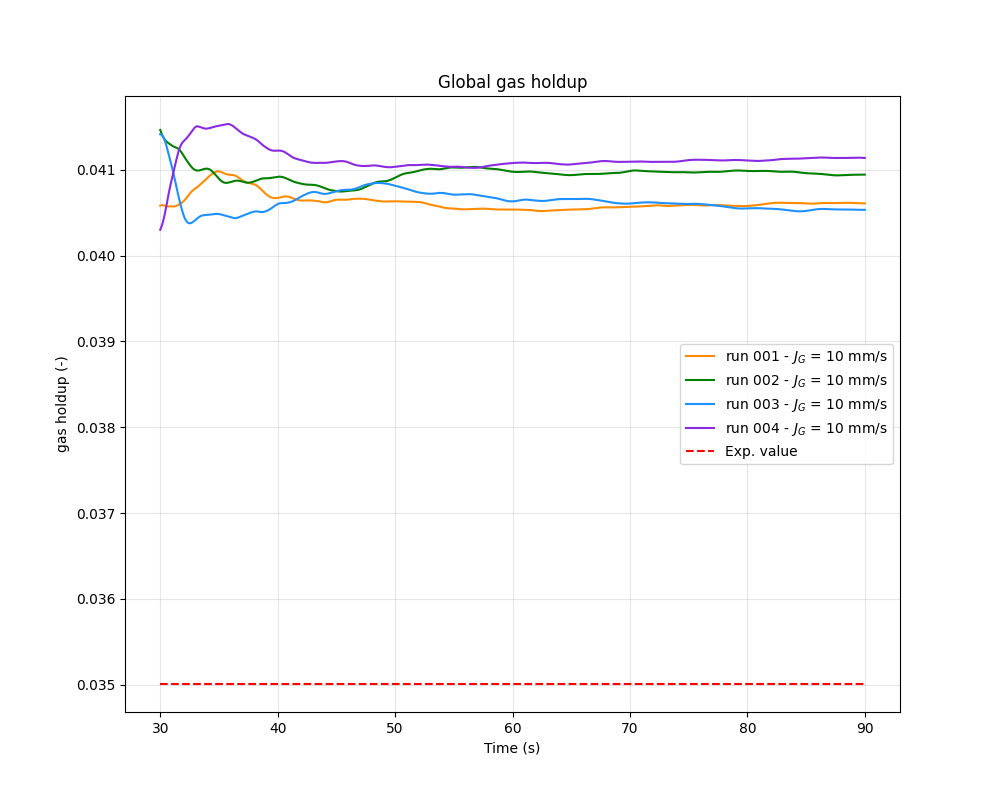
\includegraphics[width=0.5\textwidth]{Images/graphs/mesh/holdUp10.png}
    \caption{Averaged holdup for different meshes}
    \label{fig:holdup_mesh}
\end{figure}

\begin{figure}[H]
    \centering
    \subfloat[h = 8 cm]{
        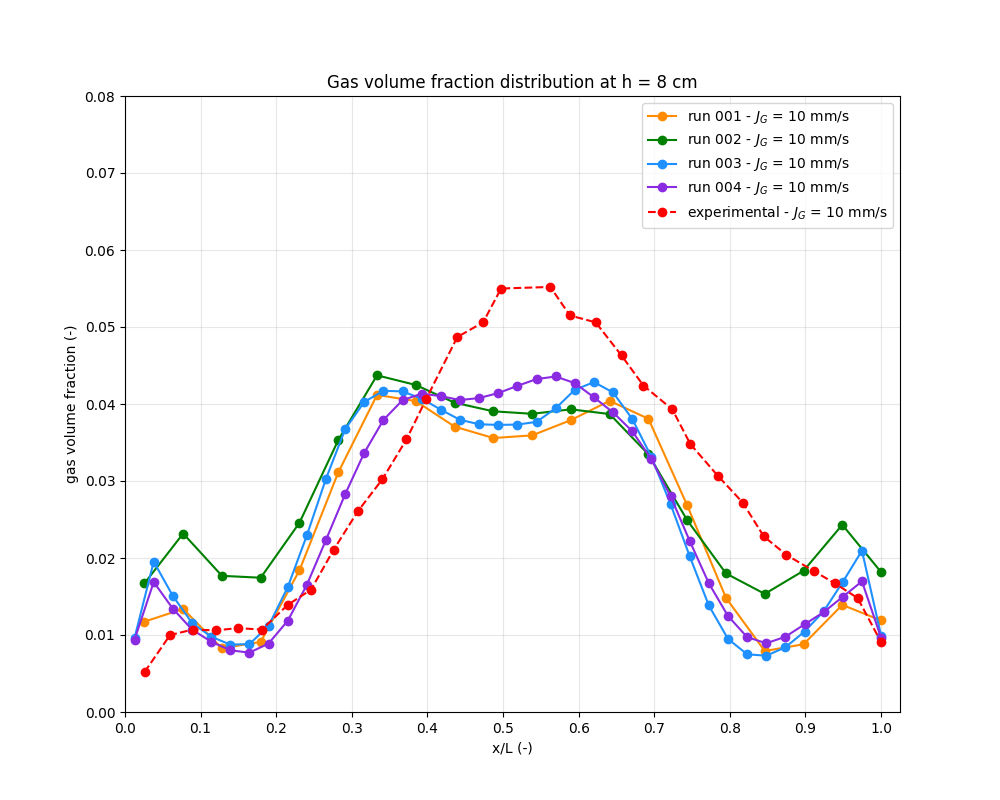
\includegraphics[scale=0.35]{Images/graphs/mesh/surfacesJ10h8.png}
    }
    \subfloat[h = 63 cm]{
        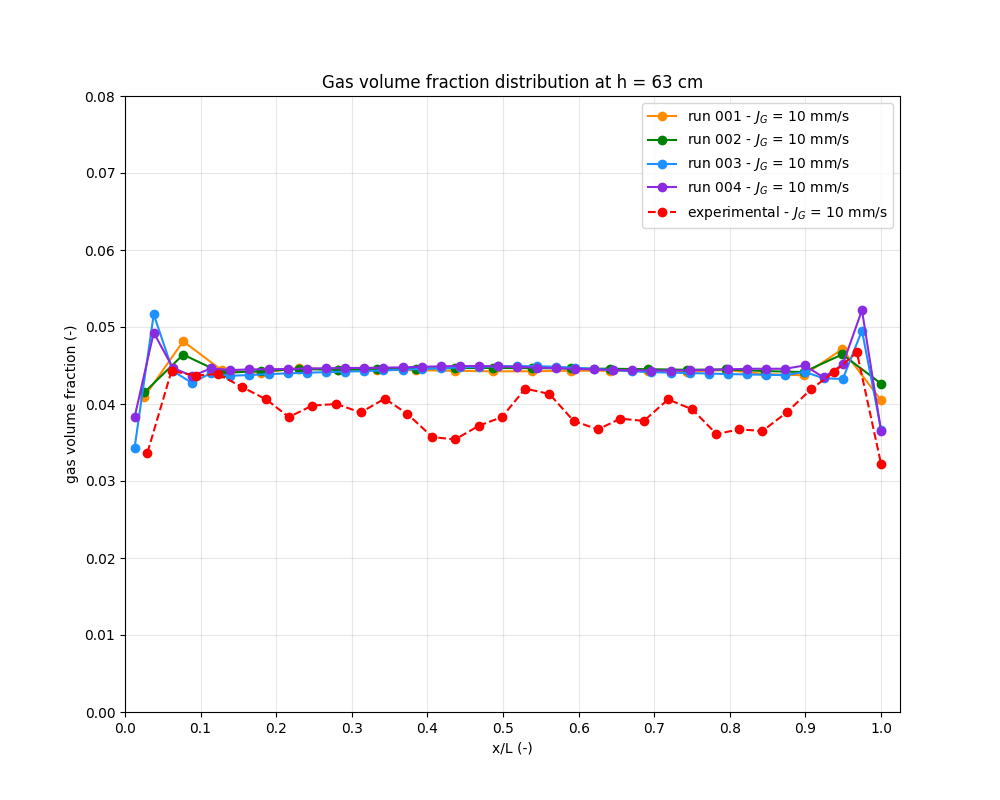
\includegraphics[scale=0.35]{Images/graphs/mesh/surfacesJ10h63.png}
    }
    \caption[]{Gas volume fraction horizontal distribution at different heights for different meshes}
    \label{fig:alpha_mesh}
\end{figure}

\subsection{Time sensitivity}
\label{sub:time_sensitivity}

\begin{table}[H]
    \centering 
    \begin{tabular}{|p{8em} c |}
    \hline
    \rowcolor{bluePoli!40}
     & \textbf{$\Delta t$} \T\B \\
    \hline \hline
    \textbf{run006} & 0.0025 \T\B \\
    \textbf{run001} & 0.005 \T\B \\
    \textbf{run005} & 0.010 \T\B \\
    \hline
    \end{tabular}
    \\[10pt]
    \caption{Time steps}
    \label{table:time_steps}
\end{table}

\begin{figure}[H]
    \centering
    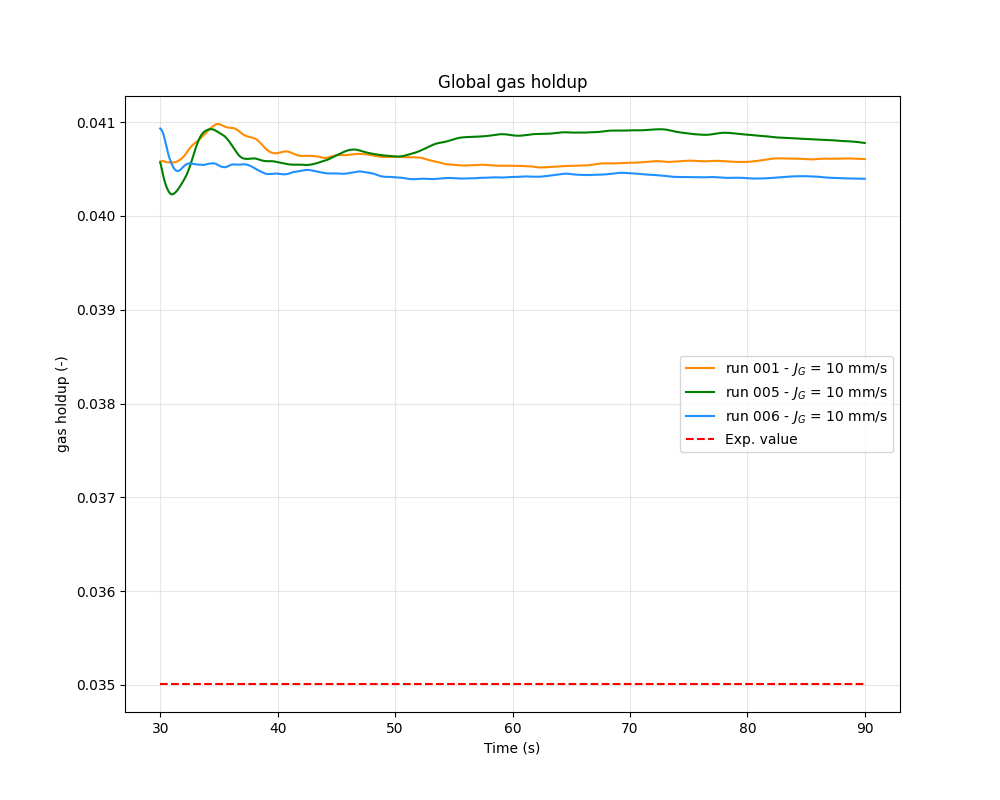
\includegraphics[width=0.5\textwidth]{Images/graphs/time/holdUp10.png}
    \caption{Averaged holdup for different time steps}
    \label{fig:holdup_time}
\end{figure}

\begin{figure}[H]
    \centering
    \subfloat[h = 8 cm]{
        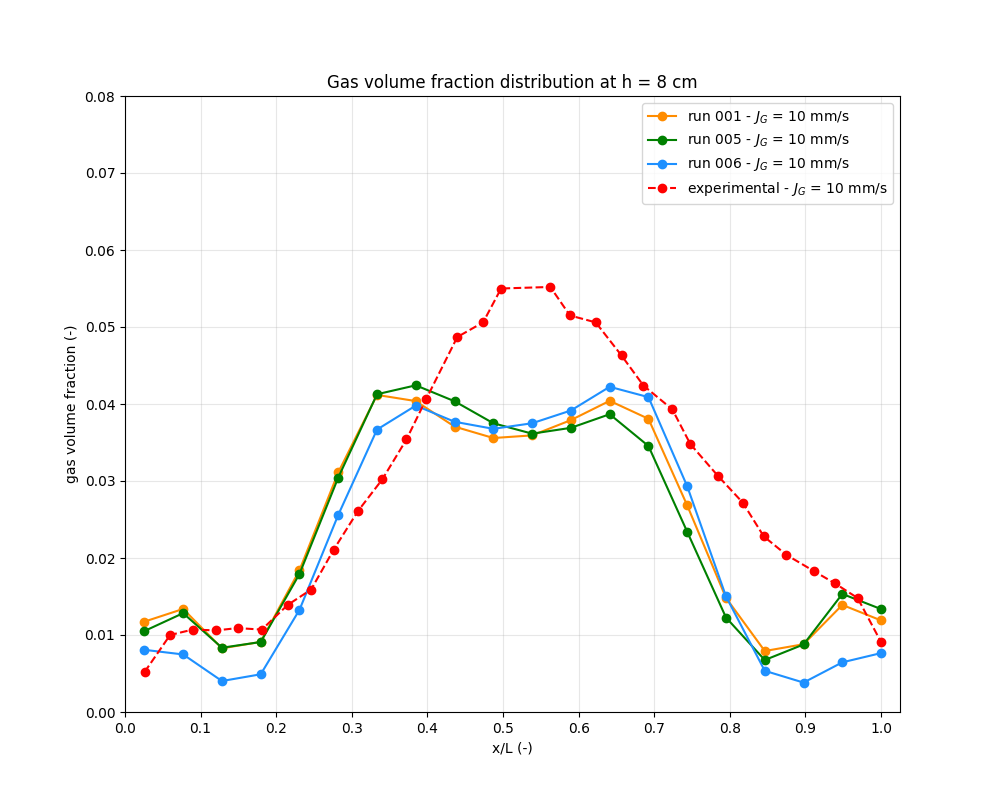
\includegraphics[scale=0.35]{Images/graphs/time/surfacesJ10h8.png}
    }
    \subfloat[h = 63 cm]{
        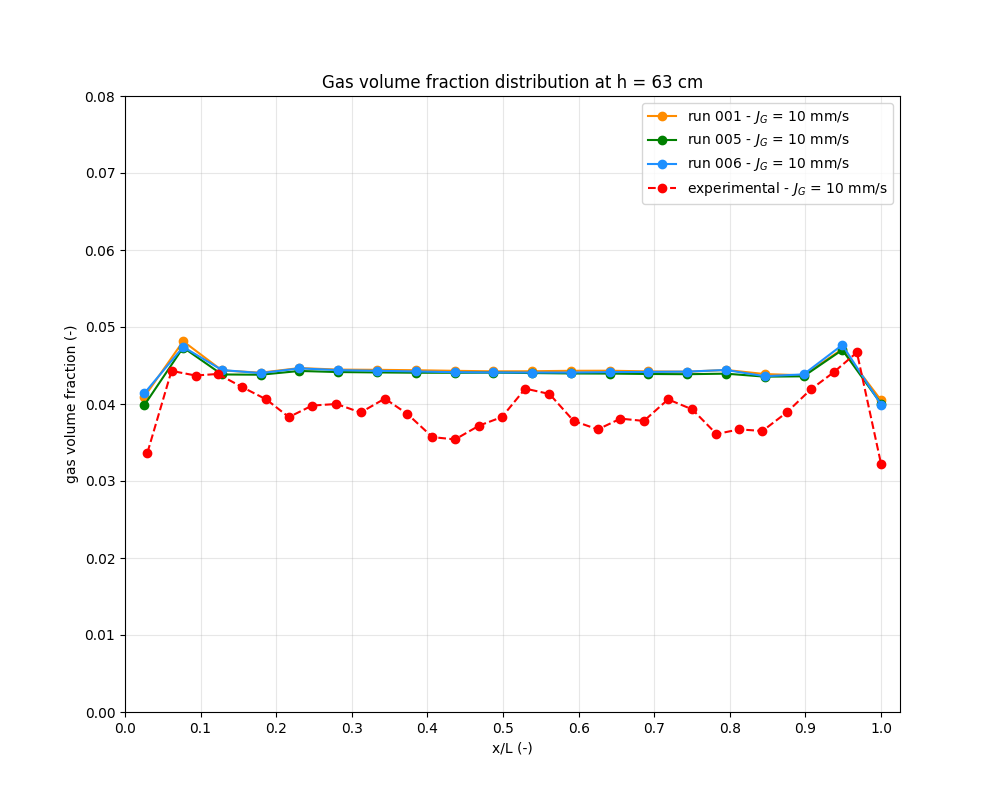
\includegraphics[scale=0.35]{Images/graphs/time/surfacesJ10h63.png}
    }
    \caption[]{Gas volume fraction horizontal distribution at different heights for different time steps}
    \label{fig:alpha_time}
\end{figure}

\subsection{Turbulence models}
\label{sub:turbulence_models}

\subsubsection{\boldmath$k-\omega$ SST Sato}
The \textit{$k-\omega$ SST Sato} model \citep{SSTSato} has originally developed to tackle the problem of heat transfer for boundary layer flows. It combines eddy-viscosity models for the momentum equations and eddy-diffusivity model for heat transer. \\
The idea behind SST model is to combine the best elements of the $k-\epsilon$ model and the $k-\omega$ model with the help of a blending function. Indeed, the $k-\epsilon$ model presents deficiencies near the wall, where fine meshes and specific near-wall treatments are required. Whereas, the $k-\omega$ model is strongly dependent of the solution to free stream values of $\omega$ outside the boundary layer.

\begin{flalign}
   \hspace{2cm}	&\frac{\partial \rho k}{\partial t} + \frac{\partial \rho U_j k}{\partial x_j} 	= \tilde{P_k} - \beta^\star \rho \omega k + \frac{\partial}{\partial x_j}			\left(\Gamma_k \frac{\partial k}{\partial x_j}\right) \label{eq:k-equation_kOmegaSSTSato} & \\
   	&\frac{\partial \rho \omega}{\partial t} + \frac{\partial \rho U_j \omega}{\partial x_j} = \frac{\gamma}{\nu_t}P_k - \beta \rho \omega^2 + \frac{\partial}{\partial x_j}\left(\Gamma_\omega \frac{\partial \omega}{\partial x_j}\right) + (1-F_1)2\rho\sigma_{\omega 2}\frac{1}{\omega}\frac{\partial k}{\partial x_j}\frac{\partial \omega}{\partial x_j} \label{eq:omega-equation_kOmegaSSTSato}&
\end{flalign}
with
\begin{flalign}
   \hspace{2cm}	& \Gamma_k = \mu + \frac{\mu_t}{\sigma_k}, \hspace{0.1cm} \Gamma_\omega = \mu + \frac{\mu_t}{\sigma_\omega}, \hspace{0.1cm} P_k = \tau_{ij}\frac{\partial U_i}{\partial x_j}, \hspace{0.1cm} \tilde{P_k} = \min(P_k;c_l\epsilon), \hspace{0.1cm} \mu_t = \rho\frac{a_1k}{\max(a_1\omega; S \cdot F_2)} &
\end{flalign}
The coefficients, $\phi$ of the model are function of $F_1$: $\phi = F_1 \phi_1 + (1-F_1)\phi_2$, where $\phi_1$ and $\phi_2$ stand for the coefficients fo the $k-\omega$ and the $k-\epsilon$ model rispectively:
\begin{flalign}
   \hspace{2cm}	& \sigma_{k1}=1.176, \hspace{0.1cm} \sigma_{\omega 1}=2.000, \hspace{0.1cm} \kappa = 0.41, \hspace{0.1cm} \gamma_1 = 0.5532, \hspace{0.1cm} \beta_1 = 0.0750, \hspace{0.1cm} \beta^\star = 0.09, \hspace{0.1cm} c_1 = 10 & \\
   & \sigma_{k2}=1.00, \hspace{0.1cm} \sigma_{\omega 2}=1.168, \hspace{0.1cm} \kappa = 0.41, \hspace{0.1cm} \gamma_2 = 0.4403, \hspace{0.1cm} \beta_2 = 0.0828, \hspace{0.1cm} \beta^\star = 0.09&
\end{flalign}
with
\begin{flalign}
   \hspace{2cm}	& F_1 = \tanh &
\end{flalign}
Here, the absolute value of the strain rate, S, is used in the definition of the eddy viscosity instead of the vorticity in order to increase the generality of the method beyond aerodynamic applications.\\
The turbulent heat flux vector is modelled with the help of a turbulent diffusivity:





















\subsubsection{Lahey $k-Epsilon$}

\subsubsection{Mixture $k-Epsilon$}

\begin{table}[H]
    \centering 
    \begin{tabular}{|p{8em} c |}
    \hline
    \rowcolor{bluePoli!40}
    & \textbf{Turbulence model} \T\B \\
    \hline \hline
    \textbf{run001} & kOmegaSSTSato \T\B \\
    \textbf{run007} & LaheyKEpsilon \T\B \\
    \textbf{run008} & mixtureKEpsilon \T\B \\
    \hline
    \end{tabular}
    \\[10pt]
    \caption{Turbulence models}
    \label{table:turbulence_models}
\end{table}

\begin{figure}[H]
    \centering
    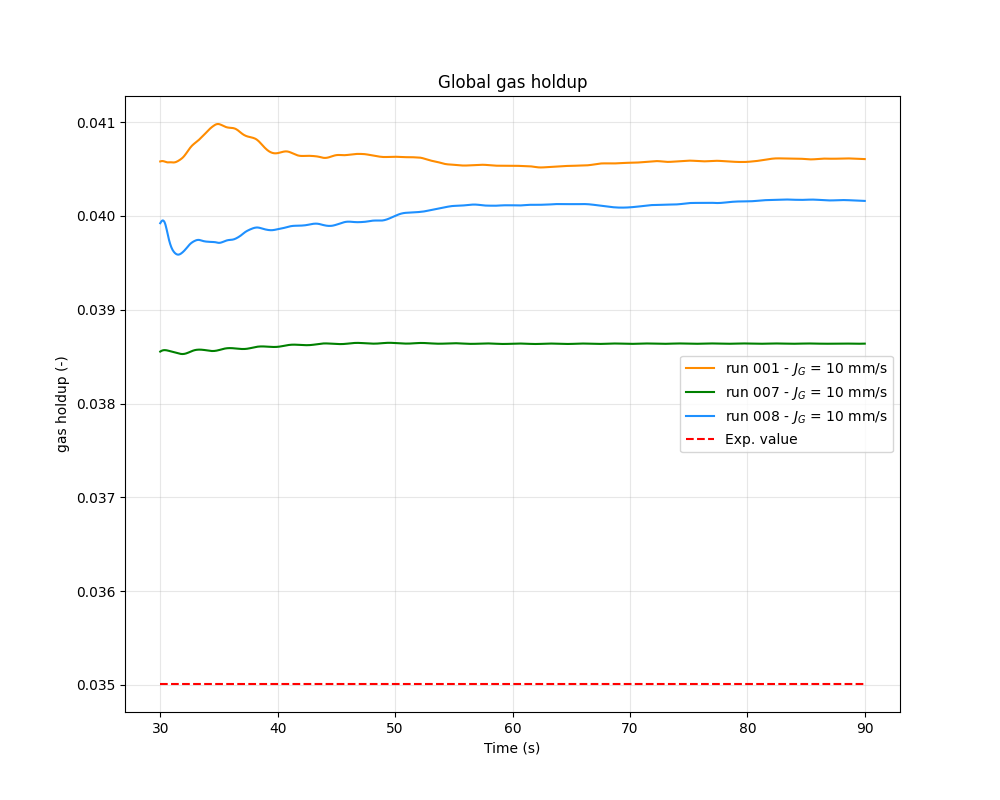
\includegraphics[width=0.5\textwidth]{Images/graphs/turbmodel/holdUp10.png}
    \caption{Averaged holdup for different turbulence models}
    \label{fig:holdup_turbmodel}
\end{figure}

\begin{figure}[H]
    \centering
    \subfloat[h = 8 cm]{
        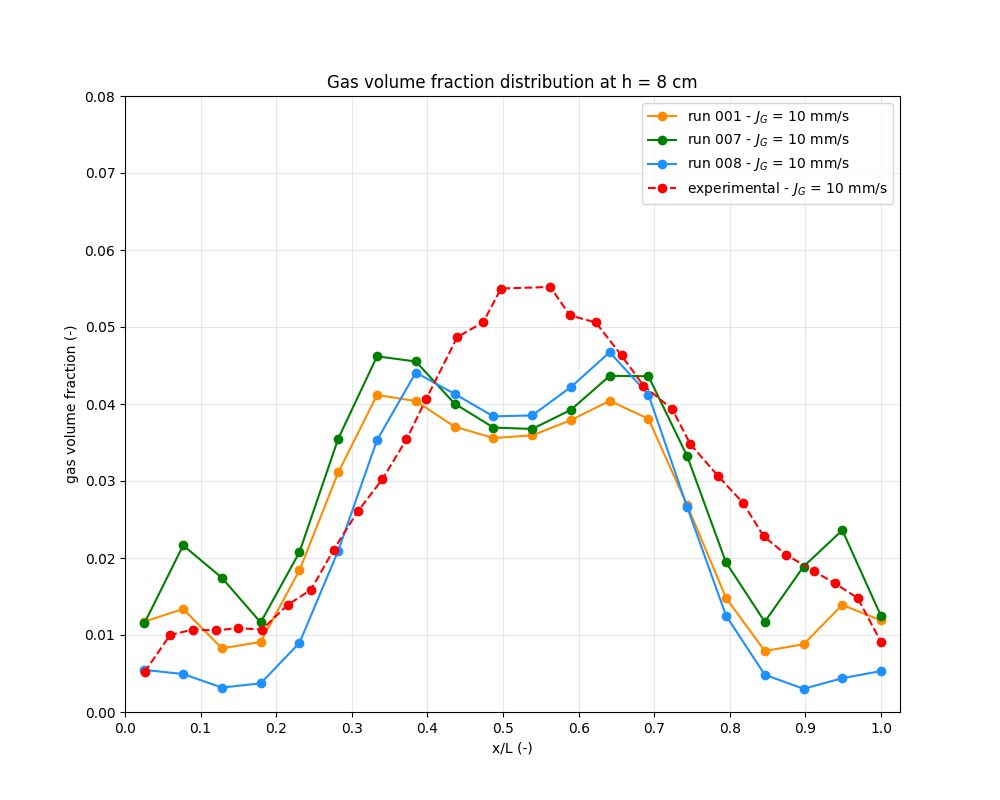
\includegraphics[scale=0.35]{Images/graphs/turbmodel/surfacesJ10h8.png}
    }
    \subfloat[h = 63 cm]{
        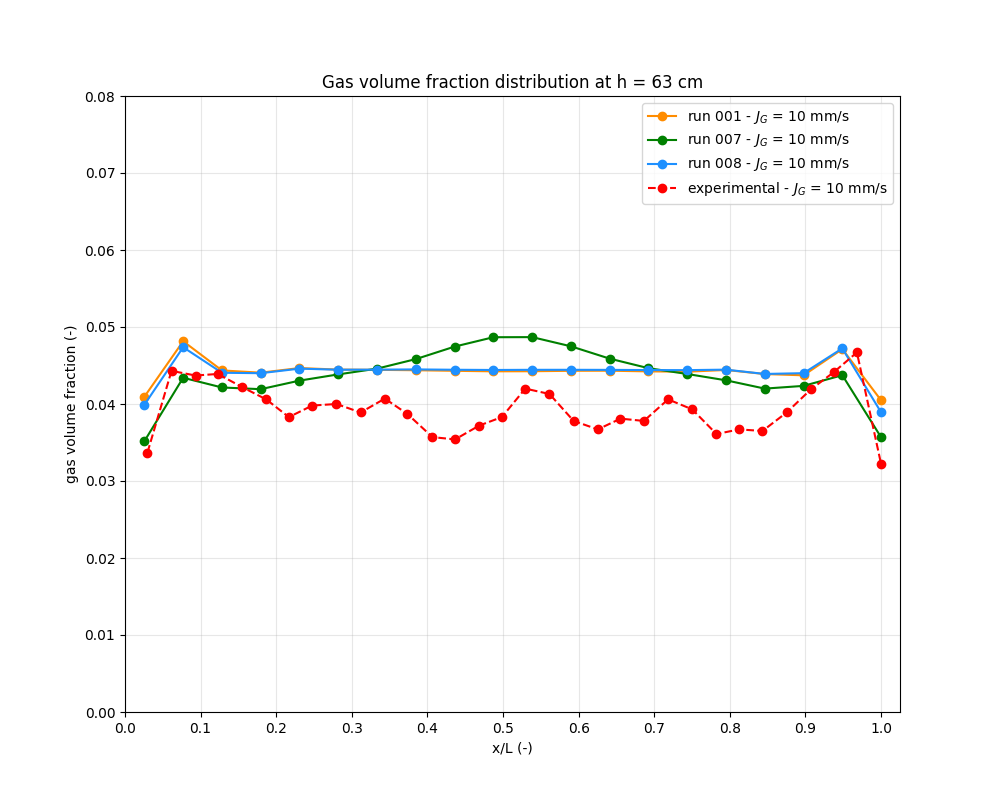
\includegraphics[scale=0.35]{Images/graphs/turbmodel/surfacesJ10h63.png}
    }
    \caption[]{Gas volume fraction horizontal distribution at different heights for different turbulence models}
    \label{fig:alpha_turbmodel}
\end{figure}

\subsection{Drag models}
\label{sub:drag_models}

\subsubsection{IshiiZuber}


\begin{table}[H]
    \centering 
    \begin{tabular}{|p{8em} c |}
    \hline
    \rowcolor{bluePoli!40}
    & \textbf{Drag model} \T\B \\
    \hline \hline
    \textbf{all runs} &  \T\B \\
    \hline
    \end{tabular}
    \\[10pt]
    \caption{Drag models}
    \label{table:drag_models}
\end{table}

\subsection{Lift models}
\label{sub:lift_models}

\subsubsection{Tomiyama}

\subsubsection{Moraga}

\begin{table}[H]
    \centering 
    \begin{tabular}{|p{8em} c |}
    \hline
    \rowcolor{bluePoli!40}
    & \textbf{Lift model} \T\B \\
    \hline \hline
    \textbf{run009} & None \T\B \\
    \textbf{run001} & Tomiyama \T\B \\
    \textbf{run010} & Moraga \T\B \\
    \hline
    \end{tabular}
    \\[10pt]
    \caption{Lift models}
    \label{table:lift_models}
\end{table}

\begin{figure}[H]
    \centering
    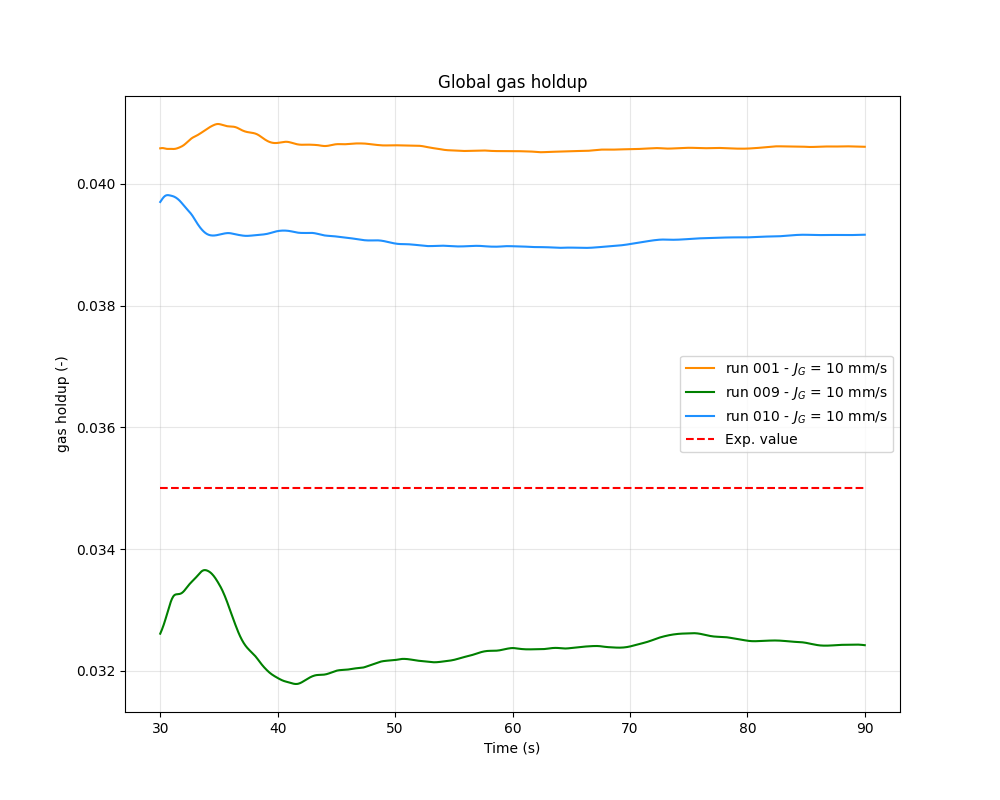
\includegraphics[width=0.5\textwidth]{Images/graphs/lift/holdUp10.png}
    \caption{Averaged holdup for different lift models}
    \label{fig:holdup_lift}
\end{figure}

\begin{figure}[H]
    \centering
    \subfloat[h = 8 cm]{
        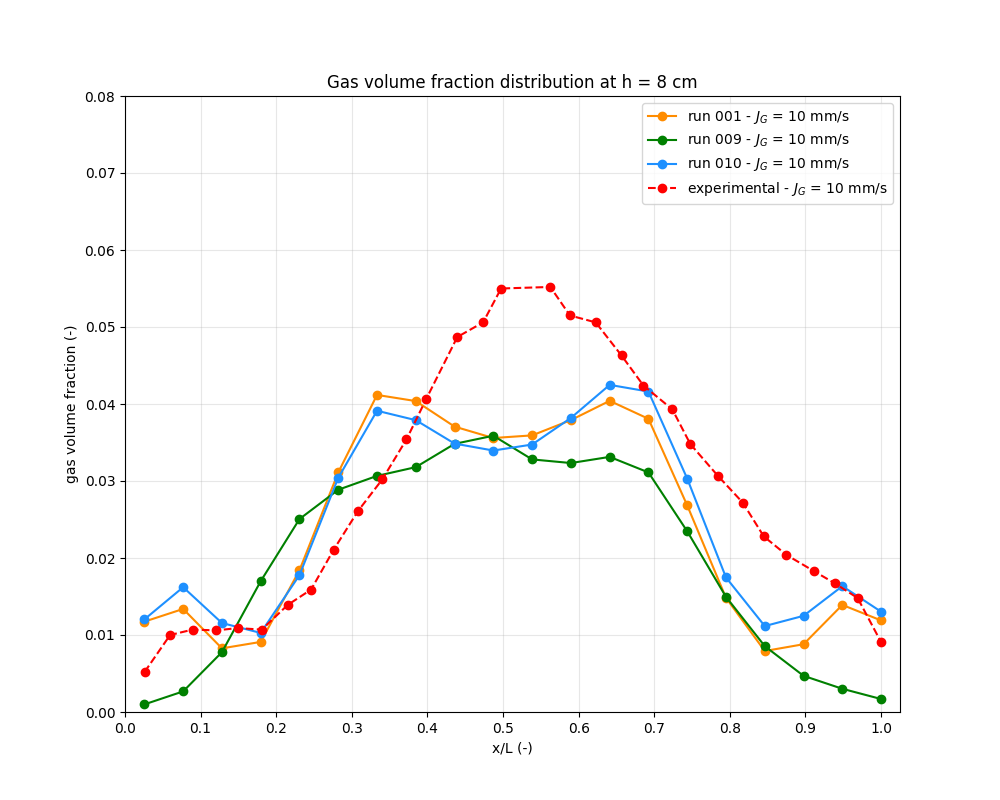
\includegraphics[scale=0.35]{Images/graphs/lift/surfacesJ10h8.png}
    }
    \subfloat[h = 63 cm]{
        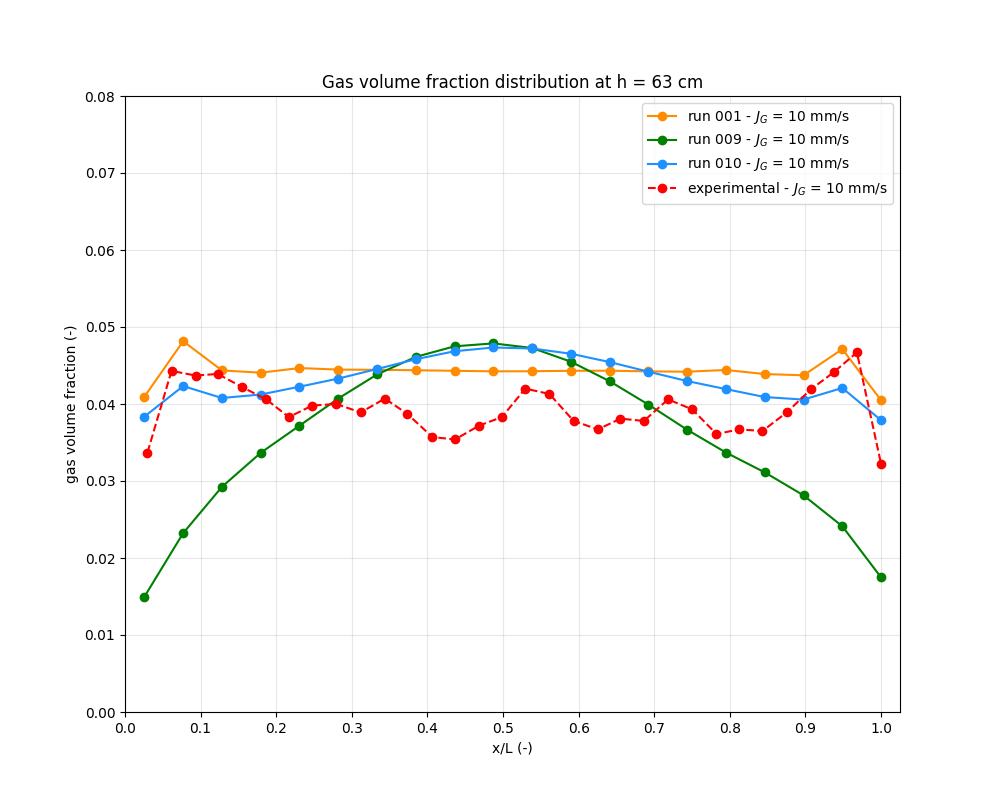
\includegraphics[scale=0.35]{Images/graphs/lift/surfacesJ10h63.png}
    }
    \caption[]{Gas volume fraction horizontal distribution at different heights for different lift models}
    \label{fig:alpha_lift}
\end{figure}

\subsection{Turbulent dispersion models}
\label{sub:turbulent_dispersion_models}

\subsubsection{Burns}

\subsubsection{LopezDeBertodanonone}

\begin{table}[H]
    \centering 
    \begin{tabular}{|p{8em} c |}
    \hline
    \rowcolor{bluePoli!40}
    & \textbf{Turbulent dispersion model} \T\B \\
    \hline \hline
    \textbf{run001} & None \T\B \\
    \textbf{run011} & Burns \T\B \\
    \textbf{run012} & LopezDeBertodanonone \T\B \\
    \hline
    \end{tabular}
    \\[10pt]
    \caption{Turbulent dispersion models}
    \label{table:turbulent_dispersion_models}
\end{table}

\begin{figure}[H]
    \centering
    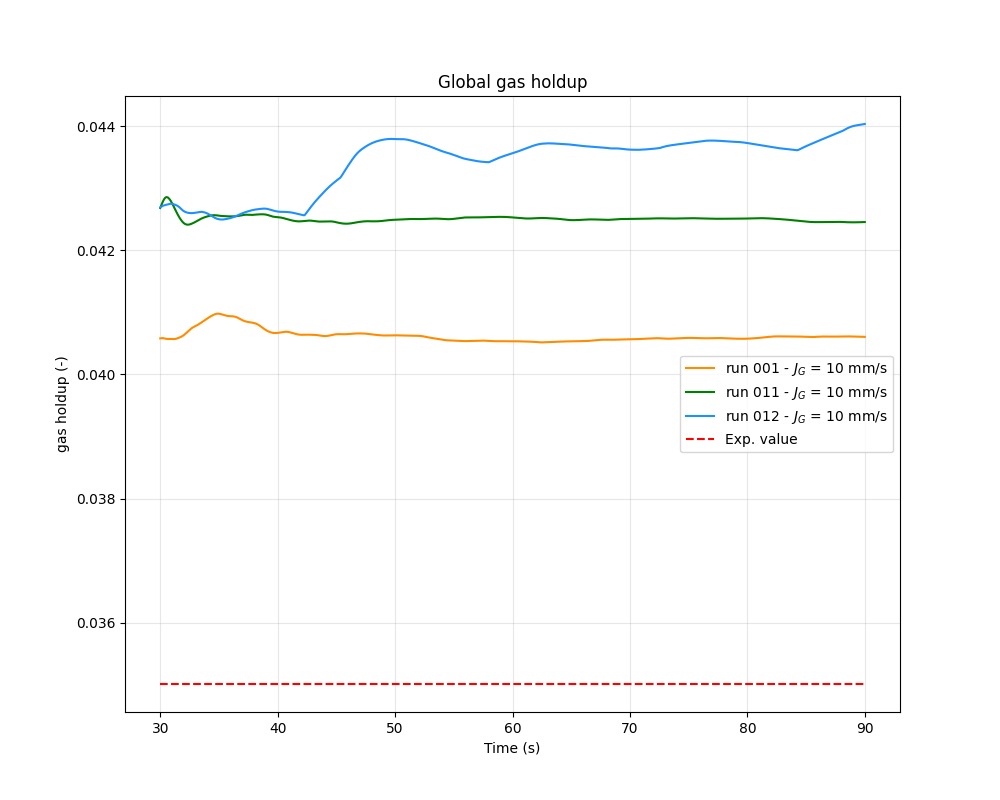
\includegraphics[width=0.5\textwidth]{Images/graphs/turbdisp/holdUp10.png}
    \caption{Averaged holdup for different turbulent dispersion models}
    \label{fig:holdup_turbdisp}
\end{figure}

\begin{figure}[H]
    \centering
    \subfloat[h = 8 cm]{
        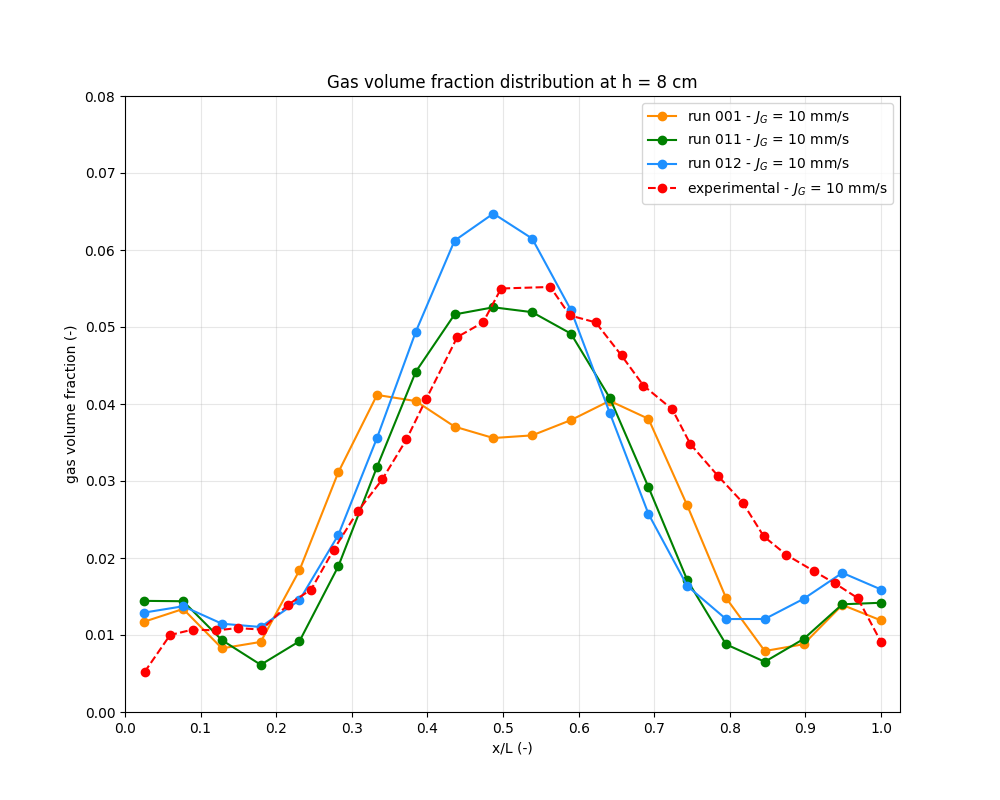
\includegraphics[scale=0.35]{Images/graphs/turbdisp/surfacesJ10h8.png}
    }
    \subfloat[h = 63 cm]{
        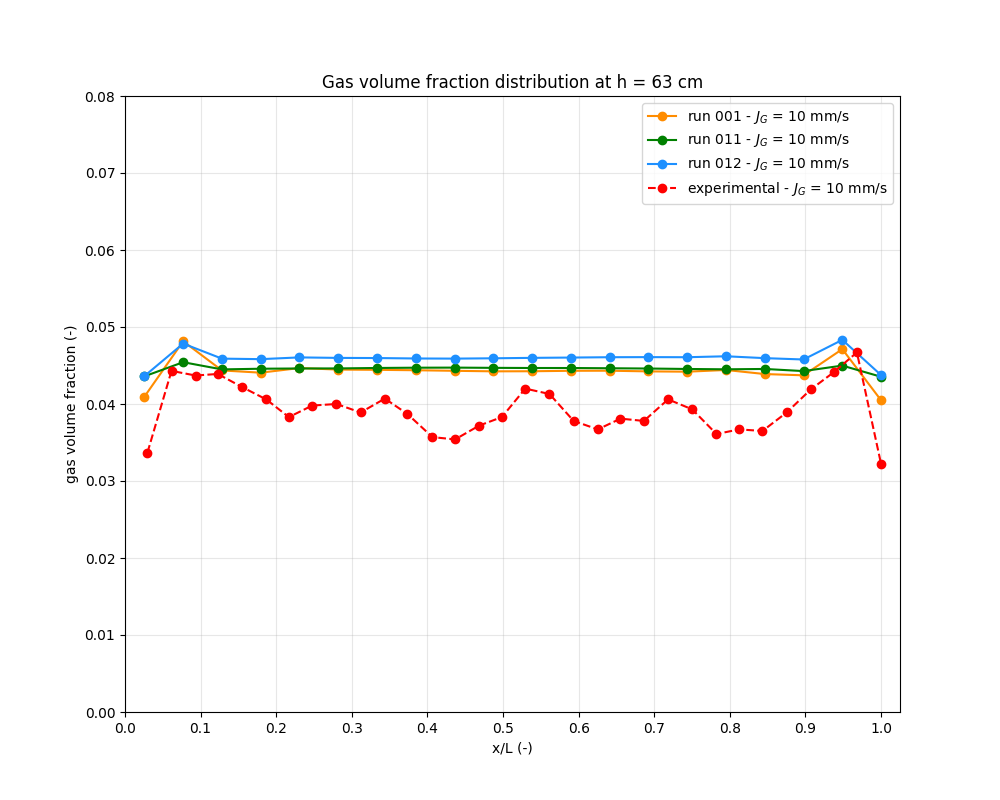
\includegraphics[scale=0.35]{Images/graphs/turbdisp/surfacesJ10h63.png}
    }
    \caption[]{Gas volume fraction horizontal distribution at different heights for different turbulent dispersion models}
    \label{fig:alpha_turbdisp}
\end{figure}

\subsection{Wall lubrication models}
\label{sub:wall_lubrication_models}

\subsubsection{Antal}

\subsubsection{Frank}

\begin{table}[H]
    \centering 
    \begin{tabular}{|p{8em} c |}
    \hline
    \rowcolor{bluePoli!40}
    & \textbf{Wall lubrication model} \T\B \\
    \hline \hline
    \textbf{run001} & None \T\B \\
    \textbf{run013} & Antal \T\B \\
    \textbf{run014} & Frank \T\B \\
    \hline
    \end{tabular}
    \\[10pt]
    \caption{Wall lubrication models}
    \label{table:wall_lubrication_models}
\end{table}

\begin{figure}[H]
    \centering
    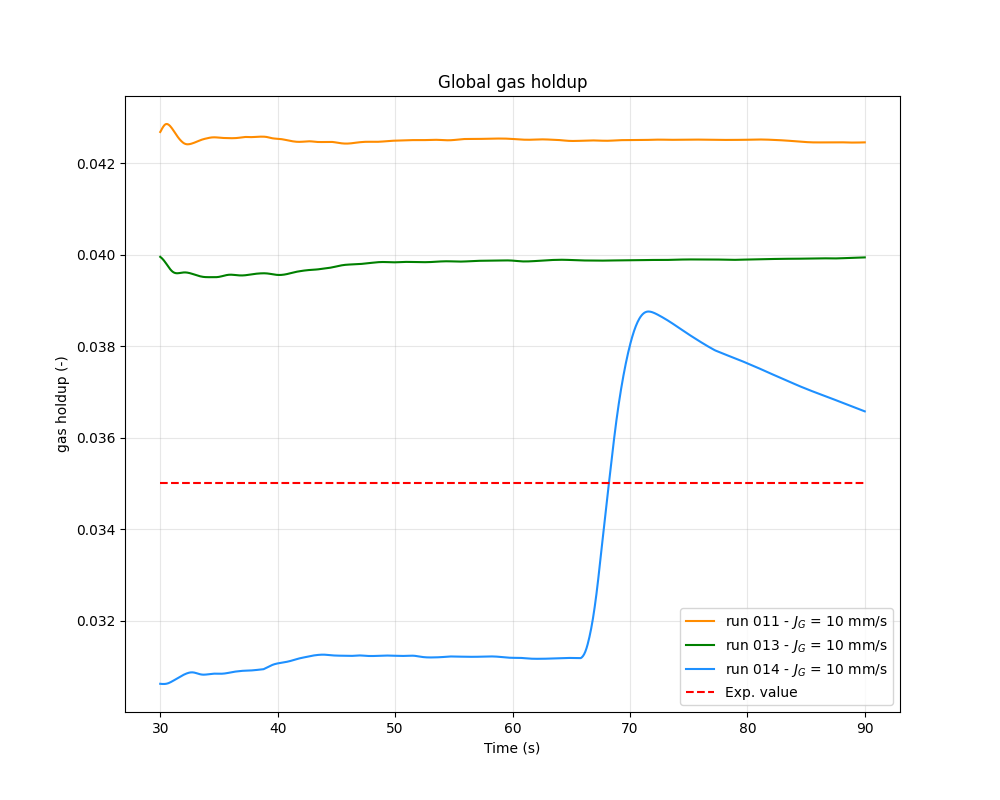
\includegraphics[width=0.5\textwidth]{Images/graphs/walllub/holdUp10.png}
    \caption{Averaged holdup for different wall lubrication models}
    \label{fig:holdup_walllub}
\end{figure}

\begin{figure}[H]
    \centering
    \subfloat[h = 8 cm]{
        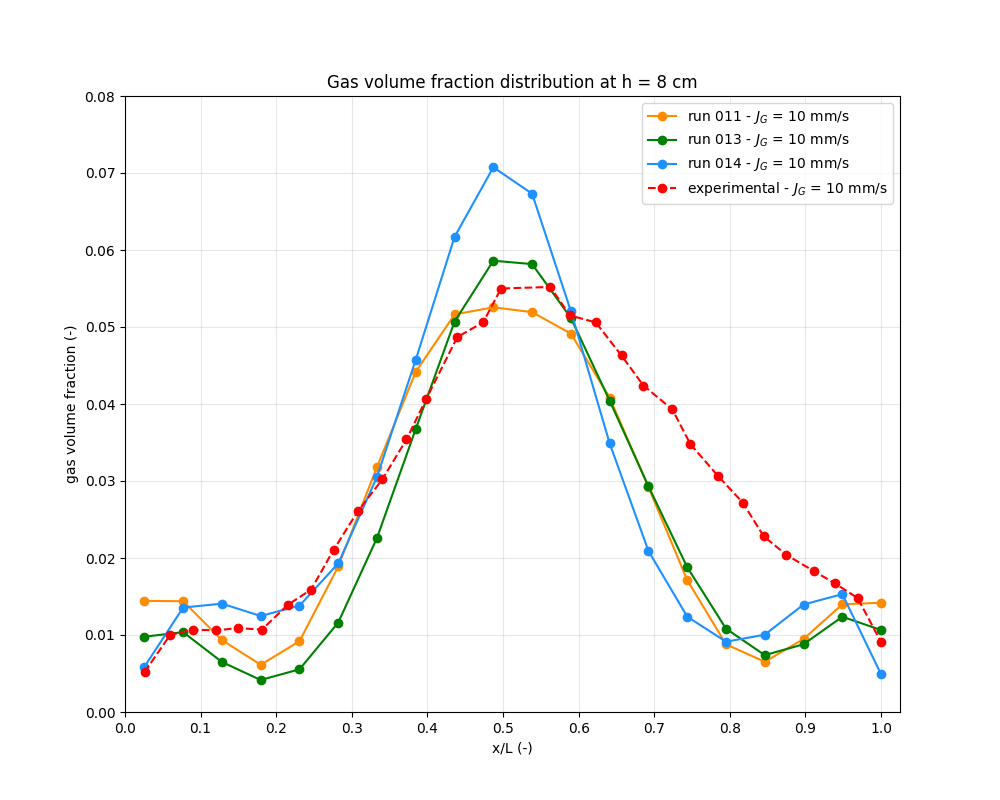
\includegraphics[scale=0.35]{Images/graphs/walllub/surfacesJ10h8.png}
    }
    \subfloat[h = 63 cm]{
        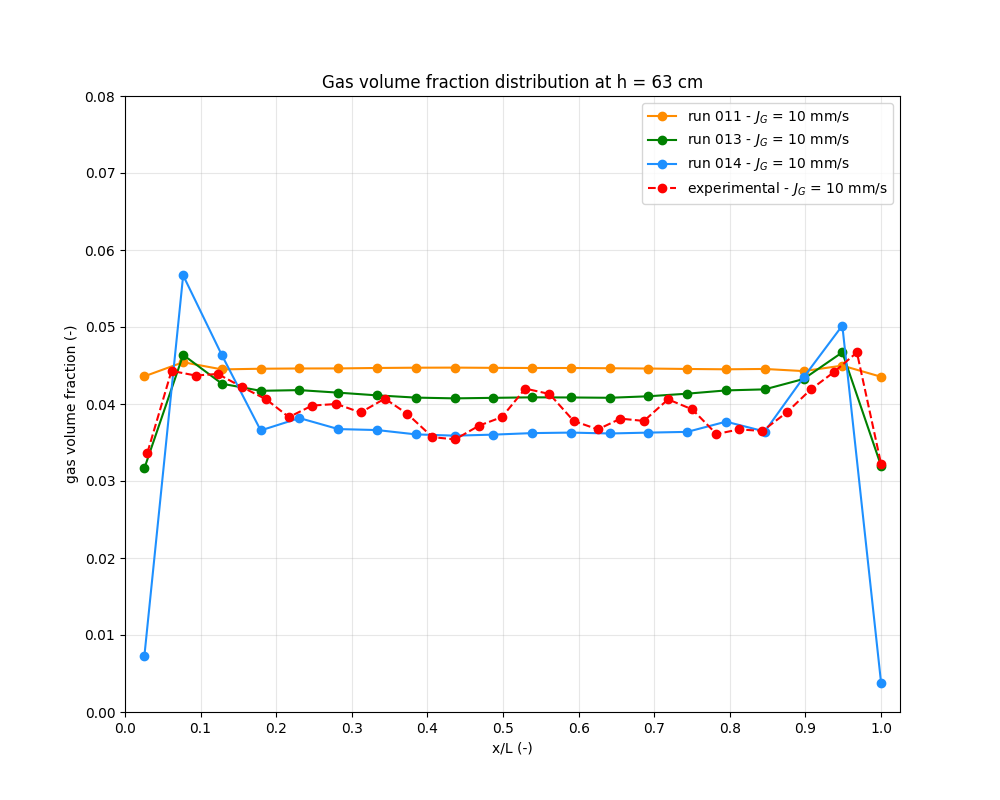
\includegraphics[scale=0.35]{Images/graphs/walllub/surfacesJ10h63.png}
    }
    \caption[]{Gas volume fraction horizontal distribution at different heights for different wall lubrication models}
    \label{fig:alpha_walllub}
\end{figure}

\subsection{Inflow velocity}
\label{sub:inflow_velocity}

\begin{table}[H]
    \centering 
    \begin{tabular}{|p{8em} c |}
    \hline
    \rowcolor{bluePoli!40}
    & \textbf{$J_{in} [mm/s]$} \T\B \\
    \hline \hline
    \textbf{run013} & 10  \T\B \\
    \textbf{run015} & 8  \T\B \\
    \textbf{run016} & 6 \T\B \\
    \hline
    \end{tabular}
    \\[10pt]
    \caption{Inflow velocities}
    \label{table:inflow_velocities}
\end{table}

\begin{figure}[H]
    \centering
    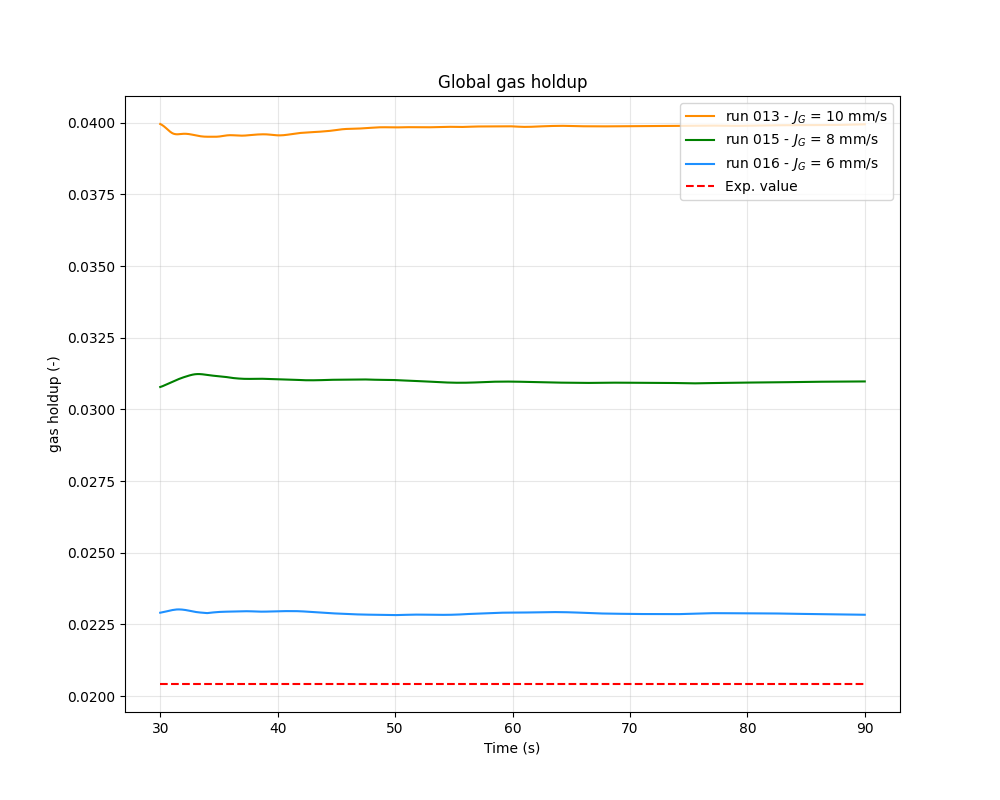
\includegraphics[width=0.5\textwidth]{Images/graphs/allj/holdUp6.png}
    \caption{Averaged holdup for different inflow velocities}
    \label{fig:holdup_inflow_velocities}
\end{figure}

\begin{figure}[H]
    \centering
    \subfloat[h = 8 cm]{
        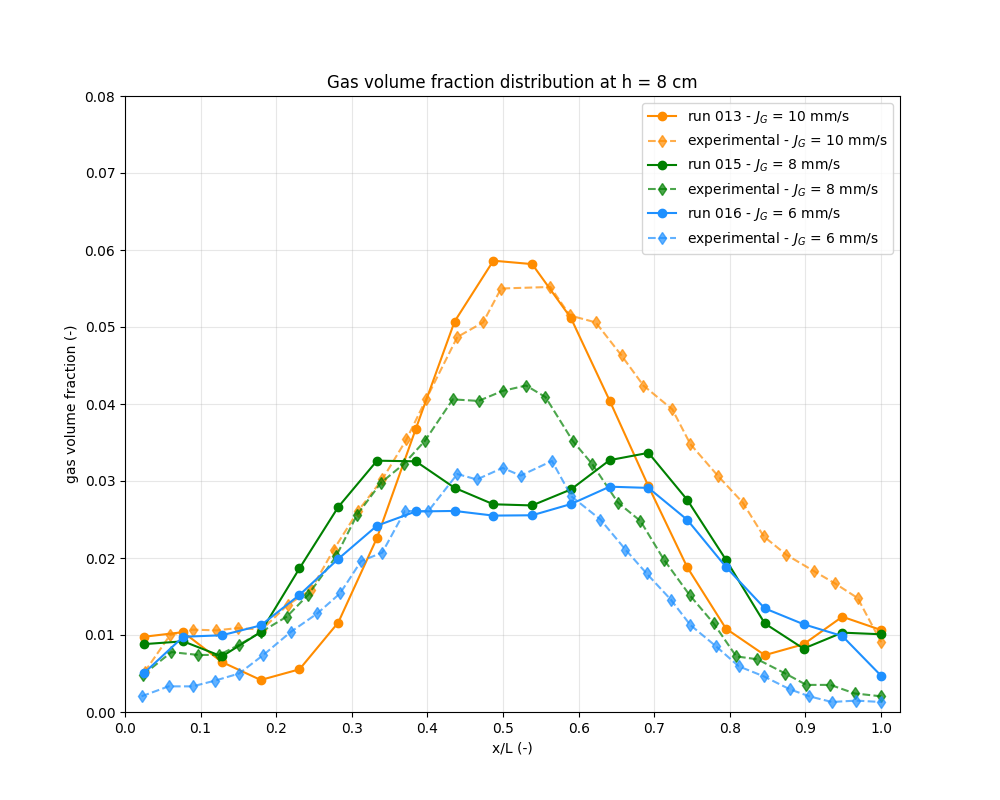
\includegraphics[scale=0.35]{Images/graphs/allj/surfacesJ6h8.png}
    }
    \subfloat[h = 63 cm]{
        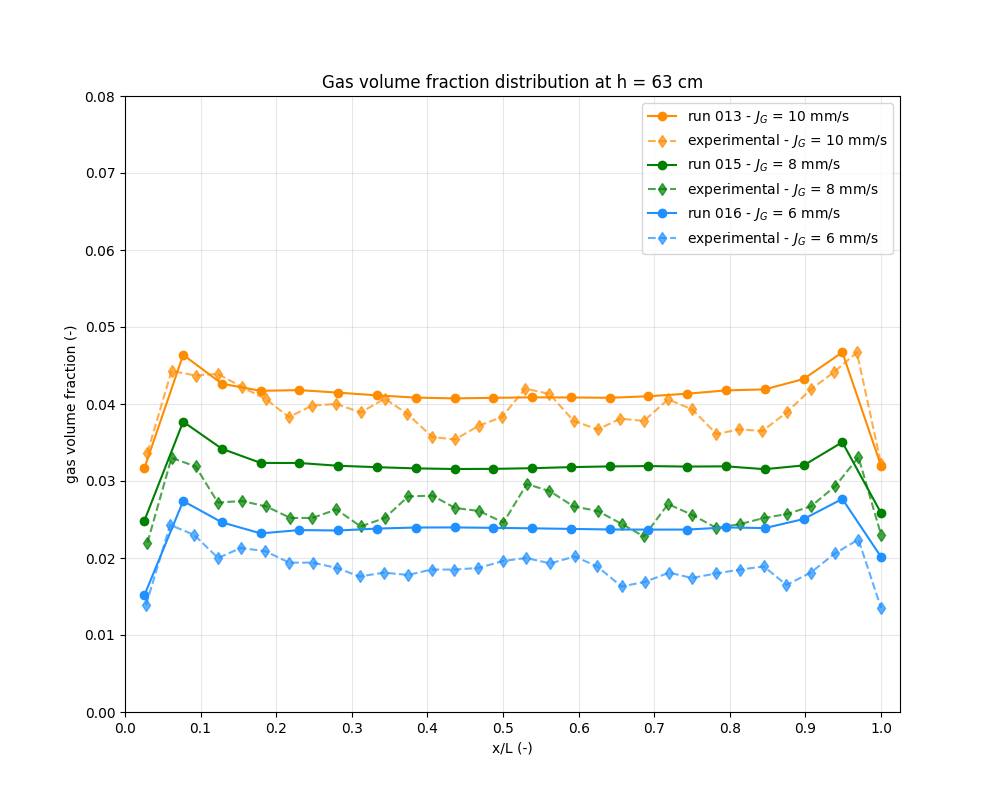
\includegraphics[scale=0.35]{Images/graphs/allj/surfacesJ6h63.png}
    }
    \caption[]{Gas volume fraction horizontal distribution at different heights for different inflow velocities}
    \label{fig:alpha_inflow_velocities}
\end{figure}

%-----------------------------------------------------------------------------
% BIBLIOGRAPHY
%-----------------------------------------------------------------------------
\bibliography{bibliography.bib}


\clearpage

%-----------------------------------------------------------------------------
% APPENDIX
%-----------------------------------------------------------------------------

\appendix
\section{Appendix A: fvModels source code for degassing boundary conditions}
\label{app:A}
\lstinputlisting[caption=fvModels source code,language=C++]{Code/fvModels}


\cleardoublepage


\end{document}
